
\section{Validation of the model}

The numerical parameters introduced in the previous section, i.e. the definition of the mesh $\delta$, and the number of droplet per domain $N$ or $N_b$ (see the definition in the previous section) need to be verified. 
Indeed, in view of carrying a numerous amount of simulations it is important to identify the minimum necessary number of droplets per domain and definition of the mesh.
Clearly, if we keep the parameter $\phi$ fixed a larger number of droplets implies a larger domain, therefore a greater numerical cost.  
Besides, the range of physical parameters needed to obtain representative closure need to be investigated to. 
Therefore, in this section we identify the ranges of numerical and physical parameters in order to obtain an efficient framework. 
The validations are all based on parameter independence arguments, meaning that we keep track of a quantity, and validate our model until the quantity is independent of the parameter. 


\tb{\subsection{Comparison with experimental or numerical simulations}
\subsubsection{Comparaison with o rdered array \citet{loisy2017buoyancy} \citep{innocenti2020direct} }
Include and launch simulations with the model of trygvason for buubles 
}
\subsection{Momentum correction}
But firstly, let's validate our last hypothesis, i.e. the \textit{momentum correction}. 
The procedure is the following, we carried out two similar simulations, one with the \textit{momentum correction} referred as the simulation $C1$, and the other without referred as $C0$.
The aim is to compare the values of the closures terms in both simulations and see if there are any differences between $C1$ and $C0$. 
They both have the following dimensionless parameters : 
$Bo = 1$, $Ga = 75$, $\mu_r  =1$, $\rho_r = 1$, $N = 5$ and $\phi = 0.15$. 
In addition, we select a number of cells per diameter $\delta = 15$ so that we intentionally create numerical error (in order to test at the limit of definition our modeling).
Also, both simulations were carried in 3 dimension. 
Of course, we expect no difference between those cases. 
\begin{figure}[h!]
    \centering
    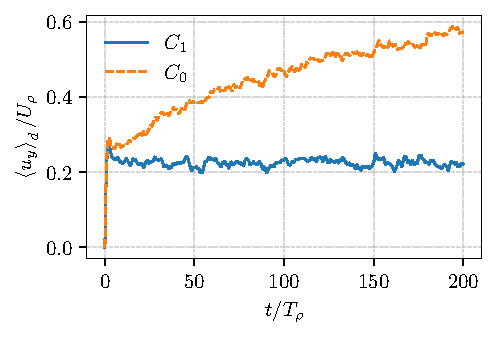
\includegraphics[height= 0.3\textwidth]{image/VALIDATION/C0C1/Ud.pdf}
    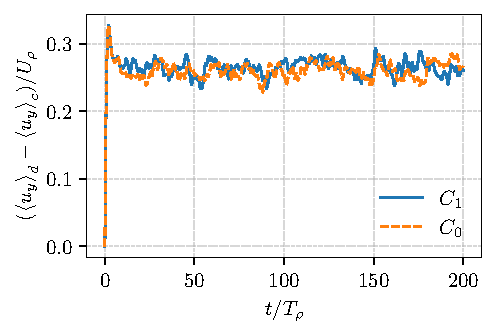
\includegraphics[height= 0.3\textwidth]{image/VALIDATION/C0C1/DeltaU.pdf}
    \caption{(left) Absolute averaged velocity of the dispersed phase along the vertical axis.
            (right) Relative velocity between the dispersed and continuous phases.
            (Dashed lines) simulation $C0$,
            (solid lines) simulation $C1$.  }
    \label{fig:VALIDATION_C0C1_1}
\end{figure}
On \ref{fig:VALIDATION_C0C1_1} we can observe the results of the two cases $C0$ and $C1$.
The (left) picture clearly shows that there is a velocity shift when no correction is applied.
Nevertheless, the two cases exhibit the same interphase velocity (see \ref{fig:VALIDATION_C0C1_1} (right)), which results in a same interphase drag force. 
The phase velocity is a term of first order, therefore it is no sensitive to the numerical parameters (e.g, number of drops per domain, number of cells per diameters).
Therefore, it is interesting to observe on \ref{fig:VALIDATION_C0C1_2}, that the similarities still holds on the first order closure terms. 
\begin{figure}[h!]
    \centering
    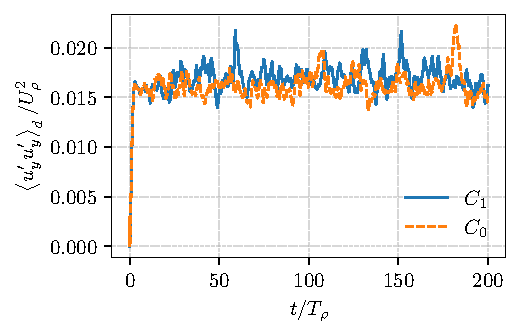
\includegraphics[height= 0.3\textwidth]{image/VALIDATION/C0C1/UpUpf.pdf}
    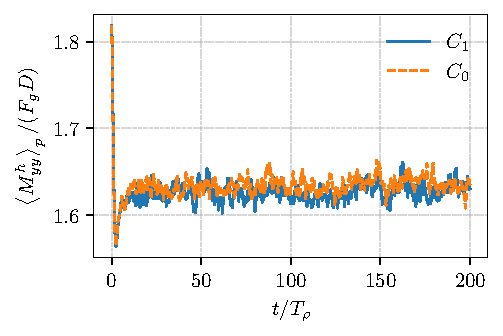
\includegraphics[height= 0.3\textwidth]{image/VALIDATION/C0C1/PA_Mh.pdf}
    \caption{(left) Fluids phase averaged fluctuation tensor.
            (right) Particular average of the first moment tensor, where $F_g$ is the buoyancy force applied on one droplet.
            (Dashed lines) simulation $C0$,
            (solid lines) simulation $C1$.  }
    \label{fig:VALIDATION_C0C1_2}
\end{figure}
Indeed, as we can remark the velocity fluctuations and the first moment are quite the same for both simulations.
It is not presented here, but all quantities remain the same thus the \textit{momentum corrector} isn't influencing any of these closures terms. 

\subsection{Number of particles per domain and definition of the mesh}

Now, let's investigate the required number of droplets per domain, $N_b$, and the minimum definition of cells per diameter of droplets $\delta$.  
\tb{Include bibliography and expectation here \ldots}
For this investigation we kept the physical parameters presented in the same section and made a double parametric analysis over $N$ and $\delta$. 
We carried out simulations for $N = 2, 3, 4, 5, 6, 7$, and for a number of cells $10 <\delta < 40$. 
In Basilisk the mesh definition is defined by a power of two, consequently depending on the size of the domain (which is fixed to keep a $\phi$ constant) the $\delta$ parameter is fixed at a power of 2 close. 
\begin{figure}[h!]
    \centering
    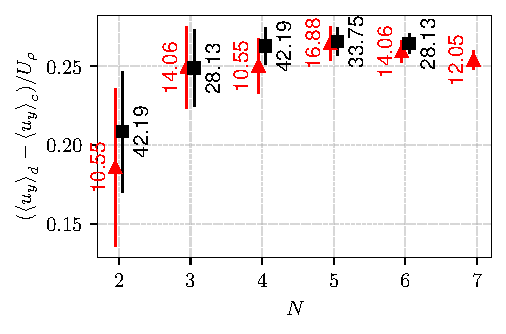
\includegraphics[height= 0.3\textwidth]{image/VALIDATION/N_and_delta/DUd.pdf}
    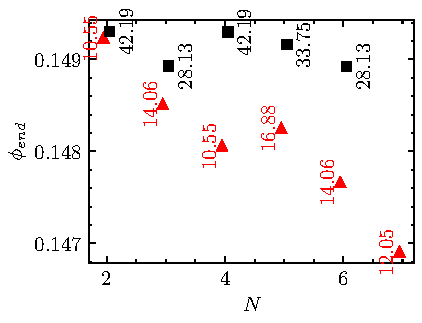
\includegraphics[height= 0.3\textwidth]{image/VALIDATION/N_and_delta/PHI.pdf}
    \caption{(left) Averaged relative velocities for both phases.
            (right) Dispersed phase volume fraction at the end of each simulation.
            The text on the side of the points is $\delta$. }
    \label{fig:VALIDATION_Nd_1}
\end{figure}
\ref{fig:VALIDATION_Nd_1}(left), illustrate clearly that the drift velocity is independent of the parameters $N_b$ and $\delta$, for $N >4$. 
On the other hand, \ref{fig:VALIDATION_Nd_1}(right), show that the volume fraction of the dispersed phase is lower for the low defined grid (red dots), due to a loss of volume during the simulation.
This doesn't mean that the solver isn't volume conservative. 
In fact, it is fund to be due to the \href{http://basilisk.fr/sandbox/fintzin/Rising-Suspension/no-coalescence.h}{no-coalescence.h} which generate fragment into the numerical domain, fragment which are deleted in the long run. 
\begin{figure}[h!]
    \centering
    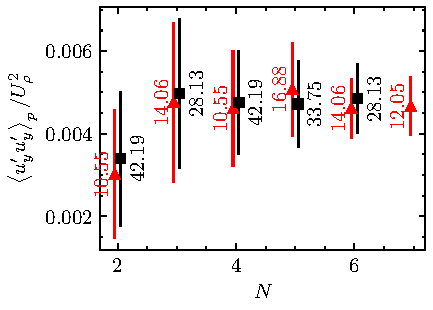
\includegraphics[height= 0.3\textwidth]{image/VALIDATION/N_and_delta/PA_UpUp.pdf}
    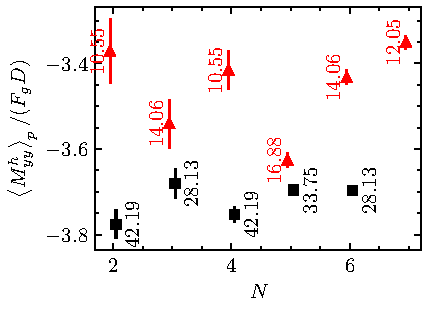
\includegraphics[height= 0.3\textwidth]{image/VALIDATION/N_and_delta/Mh.pdf}
    \caption{(left) Fluids phase averaged fluctuation tensor.
            (right) Particular average of the first moment tensor, where $F_g$ is the buoyancy force applied on one droplet. 
            The numerical values displayed alongside the dots are the number of cells per diameter.}
    \label{fig:VALIDATION_Nd_2}
\end{figure}
Now, let's look at the behavior of more \textit{complicated} closure terms. 
\ref{fig:VALIDATION_Nd_2}(left) demonstrate that the vertical component of the pseudo turbulent tensor is parameter independent rather early, independently of the grid definition. 
This fact is rather surprising but note that the standard deviation is quite high for small domain. 
On \ref{fig:VALIDATION_Nd_2}(right), we can examine the vertical component of the first moment closure term. 
It is found to be constant for all $N$, but rather inaccurate for coarse grids. 
Which makes sens since the first moment results from a local calculation of the stress over a droplet volume, unlike the other quantities which results from the averaged center of mass velocity of a droplet. 

As we have shown, the quantities presented converge for a number of droplets equivalent to $N = 4$ and $\delta = 25$. 
Thus, we validate our simulation in space, i.e. we made sure that our domain were wide enough to minimize the influence of the periodicity on our results, and in mesh definition. 
Nevertheless, at it is the number of realization that matter when carrying a particular average, it is interesting to look at the duration of the simulation.

\subsection{Time average convergence}

The aim of this study is to be able to identify the minimum required time (or number of time steps) to obtain a representative mean. 
In this set of results we made sure that all the simulations were carried for a time that is more than sufficient. 
Therefore, in this section, we observe the convergence of the mean of a quantity depending on the number of the sample of time taken through the simulation.
More specifically we define the cumulative mean of an already, space averaged quantity, $F$, as, 
$\bar{F}(t) = \int_{T_{start}}^{t} F dt$. 
Where we introduced the start of sampling time $T_{start}$, which correspond to the starting time at which we are gathering data. 
This time is chosen as the time it takes for the simulation to reach a statistically steady state.
In other worlds, it is the time it takes for the droplets to get from an inert ordered state ($t = 0$), to a fully random state, where the droplets reach their mean drifting velocity.
As, we could remark, from its high standard deviation, the most difficult quantity, difficult in the meaning that it doesn't converge rapidly, is the \textit{Reynolds} stress tensor averaged on the particular phase, namely $\pnavg{u'_yu'_y}$.
Thus, we will confirm the representativity of our simulations, by looking at the cumulative time average of this quantity. 
\begin{figure}
    \centering
    % 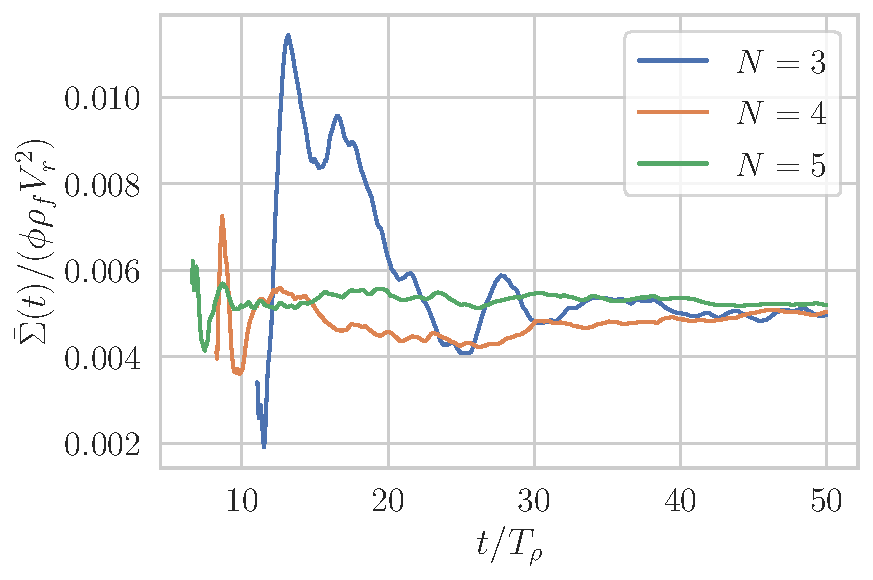
\includegraphics[height = 0.3 \textwidth]{image/VALIDATION/time/Sigma.pdf}
    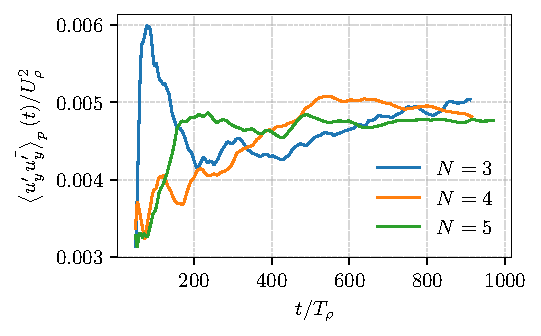
\includegraphics[height = 0.3 \textwidth]{image/VALIDATION/time/UpUp.pdf}
    \caption{Cumulative mean of the \textit{Reynolds} stress tensor. For $N = 3,4,5$ and $\delta = 25$, with $t/T_{start} = 10$.}
    \label{fig:VALIDATION_cumul_mean}
\end{figure}
From, \ref{fig:VALIDATION_cumul_mean}, it is apparent that the case where, $N=5$, has a faster convergent mean. 
Indeed, if we examine the picture, it is evident that the curve for $N=5$ reach a steady state earlier than the other ones. 
As a matter of fact, it can be perceived that the $N=5$ simulation reaches a steady mean at $t/T_\rho = 25$, while the other converge much latter. 
As a result, this study show, without surprise, that the result of the particular \textit{Reynolds} stress tends toward a steady mean faster for the simulation where $N=5$. 
In view of this it is interesting that for this range of \textit{Galileo} the time required to have significant results it $t/T_{\rho} \approx 110$, where we added the start time and $100$ inertial sampling time. 


\subsection{Asymptotic regime in low \textit{Galileo}}

Ideally we would like to cover a wide range of \textit{Galileo} numbers. 
Meaning that we need to reach both asymptotic regime, at low and high $Ga$ for any closure, if we suppose that such asymptotic regime exist. 
We limit our validation to the drag force or drift velocity closure term. 
In this section we show that in the limited range studied, i.e. $Ge \in [5,100]$, we cover enough \textit{Galileo} number to reach the low and high inertia asymptotic regime. 

First, it is interesting to see that the range of \textit{Galileo} number studied correspond to a wider range of \textit{Reynolds} numbers. 
Indeed, \ref{fig:Ga_Re} we clearly see that the computed \textit{Reynolds} numbers, based on the drift velocity, i.e. $Re = D (\cavg{\textbf{u}} - \davg{\textbf{u}}) \rho_f/\mu_f$, results in a wider range than the input \textit{Galileo} numbers. 
\begin{figure}[h!]
    \centering
    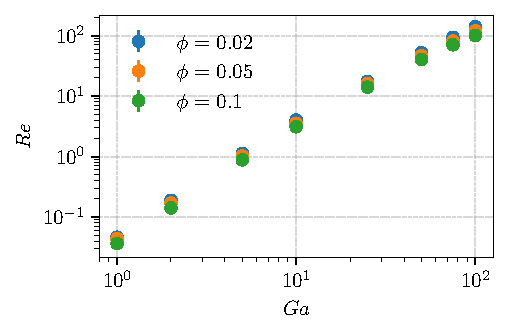
\includegraphics[height= 0.3\textwidth]{image/Dim_3/fCA/Re.pdf}
    \caption{\textit{Reynolds} number computed with the drift velocity, in terms of the \textit{Galileo} numbers.}
    \label{fig:Ga_Re}
\end{figure}
Thus, we cover both regime, inertial for $Re \approx 0.1$ and non-inertial with $Re \approx 100$. 
In order to investigate the different asymptotic regime of the drag force closure term, we plotted, in \ref{fig:f_u_f_rho}, the dimensionless drag force under two different form. 
In the first case (\ref{fig:f_u_f_rho}(left)) it is made dimensionless by the viscous material terms, namely,
\begin{equation*}
    \cavg{\textbf{f}^\mu} = \frac{\textbf{g} D^2\Delta \rho}{\mu_f |\cavg{\textbf{u}} - \davg{\textbf{u}}|}. 
\end{equation*} 
While in the other case it is made dimensionless with the inertial assumption, 
\begin{equation*}
    \cavg{\textbf{f}^\rho} = \frac{\textbf{g} D\Delta \rho}{\rho_f |\cavg{\textbf{u}} - \davg{\textbf{u}}|^2}. 
\end{equation*} 
\begin{figure}[h!]
    \centering
    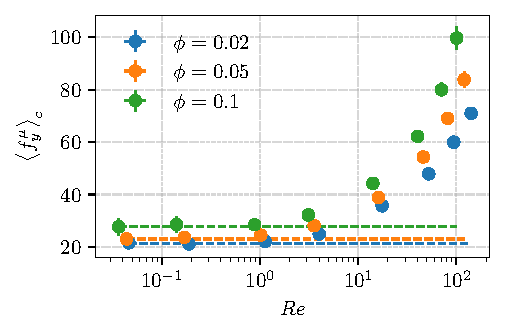
\includegraphics[height= 0.3\textwidth]{image/Dim_3/fCA/FH_Re_mu.pdf}
    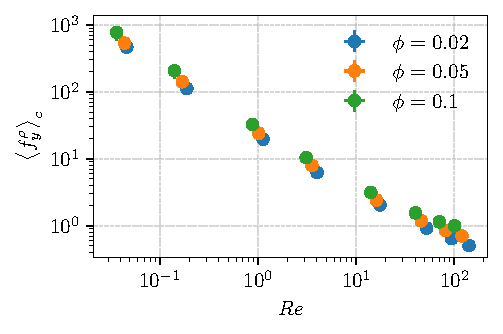
\includegraphics[height= 0.3\textwidth]{image/Dim_3/fCA/FH_rho_Re.pdf}
    \caption{(left) Non-inertial dimensionless vertical drag force term. 
             (right) Inertial dimensionless vertical drag force term. }
    \label{fig:f_u_f_rho}
\end{figure}
In \ref{fig:f_u_f_rho}(left) we can observe that $\cavg{\textbf{f}_\mu^*}$ tend to a constant value for approximately, $Re \le 1$, corresponding to a $Ga \le 5$.
Meaning, that we reach an asymptotic regime at $Ga=5$, and that it will probably tend to this same value at even lower $Re$ or $Ga$. 
However, as demonstrated by \ref{fig:f_u_f_rho} (right) the high inertial regime do not tend to a constant yet. 
Thus, no additional conclusion can be drawn so far for high inertial regime. 

In conclusion, in order to cover a wide enough range of \textit{Galileo}, we do not need to investigate $Ga<5$ since the lower \textit{Galileo} simulations, seems to behave proportionally to the case where $Ga = 5$. 
Regarding the high inertial regime, as we cannot really go above $Ga =100$ (due to the required mesh definition at higher $Ga$), we limit our study to $Ga =100$.  
Consequently, in the following simulation were carried though the range $Ga = [5,100]$, corresponding to $Re \in [1,100]$. 

\subsection{Statistical convergence}

\subsubsection{Pair PDF of presence}

In the next chapter we will see that the radial distribution function has a major importance in the closure problem. 
In order to be representative while reconstructing this function numerically, we need to gather enough sample of relative event of pairs of particles position. 
Thus, when $N$ increase, the number of particles realization of pairs of particles increase, thus we expect that $g(r)$ tends toward a constant function with increasing $N$. 
The question is, how many droplets per domain do we need so that this function is indeed representative (keeping the simulation time and time step constant) ? 
\begin{figure}[h!]
    \centering
    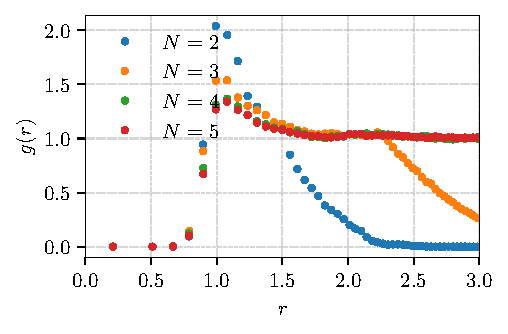
\includegraphics[height= 0.3\textwidth]{image/VALIDATION/fDist/g_r.pdf}
    \includegraphics[height= 0.3\textwidth]{image/VALIDATION/fDist/N_g_1.pdf}
    \caption{(left) Plot of the radial distribution function $g(r)$ for different $N$. 
             (right) Plot of the values of $g$ for $r =1$ in terms of the number of droplets inside the domain for different mesh definition. }
    \label{fig:g_r}
\end{figure}
On \ref{fig:g_r} (left), we see that the radial distribution function $g(r)$, tends to one with increasing $r$, which is exactly what we expect from a radial distribution function, thus it is a first validation. 
Moreover, the value of the radial distribution at $r\approx1$, is of a major importance since it is used in a closure models for the particular phase averaged stress in solid particle suspensions \citep{jackson2000dynamics}, it is also used in kinetic theory for the collision kernel modeling, \citep{fede2015monte}.
Therefore, \ref{fig:g_r} (right) we plotted the value of $g(r=1)$ for different mesh definition and number of particles per domain. 
It is evident that $g(1)$ reach a constant value above $N=4$ for a mesh definition $\delta = 25$. 

We established that the statistical distribution converged radially. 
Nevertheless, we would like to study the angular distribution in addition to the radial distribution.  
Thus, on \ref{fig:VALIDATION_fDrop_3} we show different 2D plots of this 2D distribution function. 
By comparing both plot it clearly indicates that this 2 dimensional distribution converge at $N=5$. 
\begin{figure}[h!]
    \centering
    % 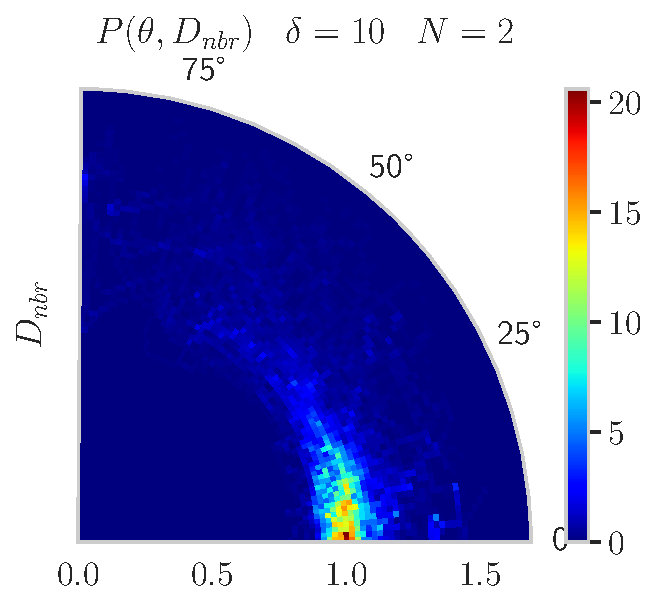
\includegraphics[height= 0.35\textwidth]{image/VALIDATION/fDrop/D_nbr_Theta_ndc_10_N_2.pdf}
    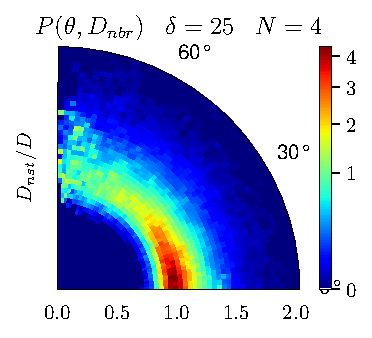
\includegraphics[height= 0.3\textwidth]{image/VALIDATION/fDrop/U_Theta_ndc_25_N_4.pdf}
    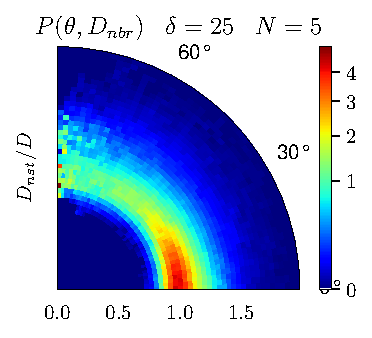
\includegraphics[height= 0.3\textwidth]{image/VALIDATION/fDrop/U_Theta_ndc_25_N_5.pdf}
    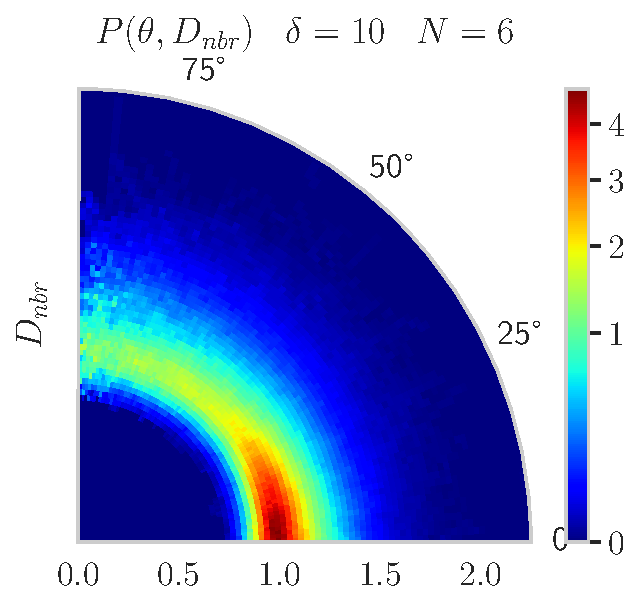
\includegraphics[height= 0.3\textwidth]{image/VALIDATION/fDrop/U_Theta_ndc_10_N_6.pdf}
    % 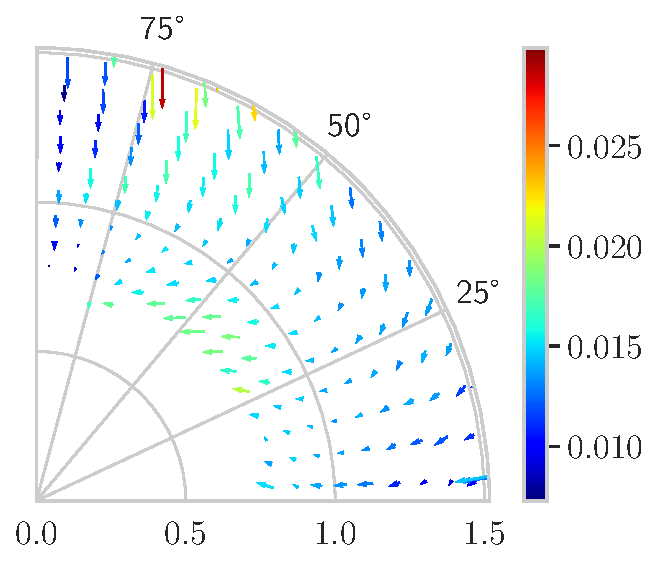
\includegraphics[height= 0.35\textwidth]{image/VALIDATION/fDrop/Dmin_Theta_Ur_uT_75_PHI_0_15.pdf}
    \caption{Radial distribution function of the nearest particle, $P(\theta, D_{nst}/D)$. 
    From $N=4$ (left) to $N=6$ simulations (right).}
    \label{fig:VALIDATION_fDrop_3}
\end{figure}
Indeed, if we look to the color bar of each plot and to the plot itself, we clearly see that the value of the PDF is the same for all $N$. 
Nevertheless, we can distinguish a small difference between $N=4$ and the others, even though it is small it deserves to be notified. 
Therefore, we consider a 2D distribution independence above a number of 64 ($N=4$) droplets per domain. 


\subsubsection{Influence of the mesh definition on nearest statistics}

Now that the required number of sample is fixed need to check out the influence of the mesh definition at the inter particle scale. 

To do so we propose to study the following a case with the following dimensionless numbers. 
We set $Ga = 75$ to be in the most disadvantageous situation. 
\begin{align}
    Ga = 75
    & \phi = 0.1
    & \mu_r =0.1 
    & \rho_r = 1.1
    & Bo = 1 
\end{align}
Finlay we test three number of cells quality, $\delta > 10$, $\delta > 25$, $\delta > 35$. 


\section{Experimental design}

From the previous few sections, we were able to identify and select relevant dimensionless parameters 
to be studied in the next chapters. 
They were deduced from parameters independence depicted in the previous few sections.
They are summaries in \ref{tab:parameters2}.
\begin{table}
    \caption{Ranges of the studied dimensionless parameters.}
    \centering
    \begin{tabular}{|c|c|c|c|c|c|c|} \hline
        $Ga$ &
        $\phi$ & 
        $Bo$ &
        $\rho_r$ &
        $\mu_r$ &
        $T_{max}/T_g$ &
        $\Delta t/T_{\sigma}$\\ \hline
        5-100
        &0.01-0.15
        & 1 
        & 1.1
        & 0.1-10
        & 500
        & 10 \\\hline
    \end{tabular}
    \label{tab:parameters2}
\end{table}
Most of the parameters have been discussed above. 
Regarding, $\phi$ we limited our study below $0.15$ because above this value bubbles or droplets instantaneously coalesce and the flow isn't dispersed anymore. 
Below $\phi =0.01$ the required domain is too wide, thus the simulations would be too expensive to carry, even though lower volume fraction would have been of interest. 
The \textit{Bond} number has been determined based on the shape of the particles. 
Indeed, we know that for extremely low $Bo$ a droplet will remain spherical. 
Thus, as for our application (see introduction of \ref{chap:avg}) we aim for spherical droplets, i.e. \textit{Bond} numbers, we need to seek for convergence toward low $Bo$. 
And as it will be shown in the results, for $Bo =1$, and this range of $Ga$, the particles remain spherical, thus we reach this asymptotic regime for low $Bo$. 
The density ratio $\rho_r = 1.1$ correspond to the ratio of our application. 
Regarding, the viscosity ratio our application (oil /water) is at $\mu_r=0.1$, but we allow our selves to explore a wider range event though we won't be able to describe entirely this dimension. 
The time of the simulation is scaled on the inertial time, $T_\rho$, as the simulations are mostly driven by inertial effect (i.e. $Ga \in [5,100]$). 
The value of $500$ inertial time has been validated empirically as can be shown by the accuracy of the previous results. 
The time step has been scaled with the capillary time in order to sample several time steps in a period of deformation of a droplet. 

In brief, the numerical parameters together with the physical ones are well validated.
Therefore, in the following chapters we carry out simulations in the restricted ranges of the parameters depicted \ref{tab:parameters2}.